\documentclass{llncs}
%
\usepackage{makeidx}  % allows for indexgeneration

\usepackage[T1,T2A]{fontenc}
\usepackage[utf8]{inputenc}
\usepackage[russian,english]{babel}
\usepackage{amsmath,amssymb}
\usepackage{subfig}
\usepackage{graphicx}
\usepackage{tabularx}
\DeclareMathOperator{\sign}{sign}
\newcolumntype{K}[1]{>{\centering\arraybackslash}p{#1}}
%
\begin{document}
%
\mainmatter              % start of the contributions
%
\title{Parallel Multi-objective Optimization on CPU Using Information Framework for Constructing Global Optimization Algorithms}
%
\titlerunning{Parallel Multi-objective Optimization}  % abbreviated title (for running head)
%                                     also used for the TOC unless
%                                     \toctitle is used
%
\author{Vladislav V. Sovrasov}
%
\authorrunning{Vladislav V. Sovrasov} % abbreviated author list (for running head)
%
%%%% list of authors for the TOC (use if author list has to be modified)
\tocauthor{Vladislav V. Sovrasov}
%
\institute{State University of Nizhny Novgorod, Nizhny Novgorod, Russia\\
\email{sovrasov.vlad@gmail.com}}

\maketitle              % typeset the title of the contribution

\begin{abstract}
В данной работе рассматривается параллельный алгоритм многокритериальной оптимизации. Рассматриваемый подход основан на применении информационно-статистического алгоритма к некоторой редуцированной однокритериальной задаче, множество глобальных оптимумов в которой совпадает с множеством слабоэффективных решений в исходной многокритериальной задаче. Последовательная версия данного метода была рассмотрена ранее. В данной работе к последовательному алгоритму многокритариальной оптимизации применяется схема распараллеливания по характеристикам, общая для всех информационно-статистических алгоритмов глобальной оптимизации. Также в работе впервые для многокритериального метода рассматривается одна из техник учёта локальных свойств оптимизируемой функции, позволяющая существенно ускорить сходимость.

\keywords{deterministi global optimization, multi-objective optimization, parallel numerical methods, derivative-free algorithms}
\end{abstract}
%
\section{Introduction}
\section{Problem Statement and Dimension Reduction}
Задача многокритериальной оптимизации ставится следующим образом:
\begin{equation}
  \label{eq:problem}
  \min\{f(y): y\in D\}, D=\{y\in \mathbb{R}^n: a_i \leqslant y_i \leqslant b_i, 1\leqslant i \leqslant n \}
\end{equation}
Будем считать, что компоненты вектор-функции (частные критерии) \(f_i(y), 1\leqslant i\leqslant m\), удовлетоворяют в \(D\) условию Липшица с константами \(L_i\):
\begin{displaymath}
\label{lip}
|f_i(y_1)-f_i(y_2)|\leqslant L_i\Vert y_1-y_2\Vert,y_1,y_2\in D,0<L_i<\infty,1\leqslant i \leqslant m
\end{displaymath}

As the solution to the problem (\ref{eq:problem}) usually accepted the set \(S(D)\in D\) of  strictly non-dominated points from the range of search, i. e.,
\begin{equation}
  \label{eq:slater}
  S(D) = \{y\in D: \nexists z\in D, f_i(z)<f_i(y),1\leqslant i \leqslant m\}
\end{equation}
which is usually referred as the set of semi-effective (or weakly effective) solutions. The conditions in the right-hand side of the definition (\ref{eq:slater}) are known as the principle of weak Pareto-optimality (or Slater's optimality principle).

The use of the evolvents \(y(x)\) i.e. the curves filling the space are a classic dimension-reduction scheme for global optimization algorithms \cite{evolvents2013}.
\begin{displaymath}
\label{cube}
\lbrace y\in R^N:-2^{-1}\leqslant y_i\leqslant 2^{-1},1\leqslant i\leqslant N\rbrace=\{y(x):0\leqslant x\leqslant 1\}
\end{displaymath}
\par
Such a mapping allows the reduction of a problem (\(\ref{eq:problem}\)) stated in a multidimensional space to solving a one-dimensional problem at the expense of worsening its properties.
In particular, the one-dimensional functions \(f_i(y(x))\) are not Lipschitzian but a Hölderian functions:
\begin{equation}
\label{eq:holder}
|f_i(y(x_1))-f_i(y(x_2))|\leqslant H_i{|x_1-x_2|}^{\frac{1}{N}},x_1,x_2\in[0,1]
\end{equation}
where the Hölder constants \(H_i\) are related to the Lipschitz constant \(L_i\) by the relation
\begin{displaymath}
H_i=4L_id\sqrt{N},d=\max\{b_i-a_i:1\leqslant i\leqslant n\}
\end{displaymath}
\par
Therefore, not limiting the generality, one can consider the solving of the
one-dimensional problem \(\min\{f(y(x)): x\in [0;1]\}\), satisfying Hölder condition. The issues of numerically building the mapping like a Peano curve and the corresponding theory have been considered in detail in \cite{evolvents2013}. Here we would note that an evolvent built numerically is an approximation to the theoretical Peano curve with a precision of the order \(2^{-m}\) where \(m\) is the building parameter of the evolvent.

\section{Description of the Parallel Algorithm With Local Refinement}
\label{sec:algorithm}
Рассмотрим схему скаляризации редуцированной задачи (\(\ref{eq:problem}\)), представленную в \cite{markinStrongin1993}. Пусть
\begin{equation}
  \varphi(x)=\max\{h(x,y):y\in [0;1]\},x\in [0;1].
\end{equation}
Рассмотрим скалярную задачу
\begin{equation}
  \label{eq:aux_problem}
  \varphi^*=\min\{\varphi(x):x\in [0;1]\}.
\end{equation}

Как показано в \cite{markinStrongin1993}, множество слабо-эффективных решений редуцированной задачи (\(\ref{eq:problem}\)) совпадает множеством глобально оптимальных решений задачи (\ref{eq:aux_problem}), т.е.
\begin{equation}
  \label{eq:s}
  S([0;1])=\{x\in [0;1]:\varphi(x)=\varphi^*\}
\end{equation}
Также в \cite{markinStrongin1993} показано, что функция \(\varphi(x)\) удовлетворяет условию Гёльдера при выполнении требований (\ref{eq:holder}). Таким образом, к функции \(\varphi(x)\) можно применить информационно-статистический алгоритм глобального поиска, чтобы решить задачу (\ref{eq:aux_problem}). Однако, \(\varphi(x)\) задаётся через оператор \(\max\{...\}\), поэтому непосредственно вычислить её затруднительно. В \cite{markinStrongin1993} приведена модификация классического информационно-статистического алгоритма \cite{mixedAlg}, в которой значения \(\varphi(x)\) вычисляются приближённо. Далее приведём модифициованную версию указанного алгоритма. Модификация заключается в использовании техники local refinement, описанной в \cite{strOptBook}(chapter 3), а также в распараллеливании по характеристикам \cite{strOptBook}(chapter 5).

Первые две итерации производятся в концевых точках \(x^0=0\) и \(x^1=1\) интервала \([0;1]\). Выбор точек \(x^{k+j}, 1\leqslant j\leqslant p\) осуществляется по правилам:

Step 1. Renumber the points in the set \(X_k=\{x^1,\dotsc,x^k\}\cup\{0\}\cup\{1\}\), which includes the boundary points of the interval \([0,1]\) as well as the points of preceding trials, by the lower indices in order of increasing coordinate values  i.e.
\begin{displaymath}
  0=x_0<x_1<\dotsc<x_{k+1}=1
\end{displaymath}

Step 2. Compute the values
\begin{equation}
\label{step2}
\mu_\nu=\max_{1\leqslant i\leqslant k}\dfrac{|f_\nu(x_i)-f_\nu(x_{i-1})|}{\Delta_i}, 1\leqslant \nu\leqslant m
\end{equation}

Step 3. Каждой точке \(x_i\), \(0\leqslant i\leqslant k\), сопоставить значение
\begin{equation}
  z_i=\max\{h(x_i,x_j):0\leqslant j\leqslant k\},
\end{equation}
где
\begin{equation}
  h(x_i,x_j)=\min\{\frac{f_\nu(x_i)-f_\nu(x_j)}{\mu_\nu}:1\leqslant \nu\leqslant m\}, 0\leqslant i,j\leqslant k
\end{equation}

Step 4. Для каждого интервала \((x_i,x_{i-1}),1\leqslant i\leqslant k\) вычислить величины
\begin{eqnarray}
  R(i) = \Delta_i + \frac{(z_i-z_{i-1})^2}{r^2\Delta_i}-\frac{z_i+z_{i-1}}{2r} \\
  R^*(i)=\frac{R(i)}{\sqrt{(z_i-z^*)(z_{i-1}-z^*)} + 1.5^{-\alpha}},
\end{eqnarray}
называемые характеристиками. При этом \(\Delta_i=(x_i-x_{i-1})^\frac{1}{N}\), \(z^*=\min\{z_i:1\leqslant i\leqslant k\}\), а \(r>1\) и \(\alpha\in [10;30]\) --- параметры метода.

Step 5. Если \(q\not=0\) и \(s \mod q\not=0 \), то характеристики \(R(i)\), \(1 \leqslant i \leqslant k + 1\), упорядочить в порядке убывания
\begin{equation*}
  R(t_1) \geqslant R(t_2) \geqslant \dots \geqslant R(t_k) \geqslant R(t_{k+1})
\end{equation*}
и выбрать \(p\) наибольших характеристик с номерами интервалов \(t_j\), \(1 \leqslant j \leqslant p\). Иначе то же самое сделать с характеристиками \(R^*(i),1\leqslant i\leqslant k+1\). Здесь \(s\) --- номер текущей итерации. \(q\) --- параметр метода, отвечающий за степень интенсивности локального уточнения. Чем меньше \(q\), тем чаще используются характеристики \(R^*\), заставляющие метод выбирать следующие точки вблизи текущего найденного минимума.

Step 6. Провести новые испытания в точках \(x^{k+j}\), \(1 \leqslant j \leqslant p\):
\begin{equation}
  x^{k+j}=\frac{x_{t_j}+x_{t_j-1}}{2} - \sign(z_{t_j} - z_{t_j-1})\frac{|z_{t_j} - z_{t_j-1}|^n}{2r}
\end{equation}
Все \(p\) испытаний на этом шаге могут быть произведены параллельно на \(p\) вычислительных устройствах.

The algorithm is terminated if the condition \(\Delta_{t_j}\leqslant \varepsilon\) is fulfilled at least for one of the numbers \(t_j\), \(1\leqslant j\leqslant p\); here \(\varepsilon >0\) is the predefined accuracy.
After the search is terminated, the set \(S(\{x^0,\dots ,x^k\})\) of all
non-dominated points of the truncated sequence \(\{x^0,\dots ,x^k\}\) is accepted as an estimation for \(S\) from (\ref{eq:s}).

The theoretical substantiation of this method when \(p=1\) and \(q=0\) is presented in \cite{strOptBook}(chapter 3). Siffitient condition of convergence is: exists an iteration such that \(r\mu_\nu \geqslant 4H_\nu,1\leqslant \nu \leqslant m\).
\section{Test Problems}
\label{sec:test_problems}
Для оценки степени ускорения сходимости модифицированного алгоритма из секции \ref{sec:algorithm} использовались следующие задачи:
\begin{enumerate}
  \item Markin-Strongin problem from \cite{markinStrongin1993}:
    \begin{equation}
      \left \{
      \begin{array}{l}
        f_1(y) = \min\{\sqrt{y_1^2+y_2^2},\sqrt{(y_1-1.5)^2+(y_2+1.5)^2}\} \\
        f_2(y)=\sqrt{(y_1+0.5)^2+(y_2-0.5)^2} \\
      \end{array}
      \right .
      y_1\in [-1;2],y_2\in [-2;1]
    \end{equation}
  \item Fonseca and Fleming problem \cite{Huband2006}:
  \begin{equation}
    \label{eq:fonseca}
    \left \{
    \begin{array}{l}
      f_{1}\left(y\right) = 1 - \exp \left(-\sum_{i=1}^{n} \left(y_{i} - \frac{1}{\sqrt{n}} \right)^{2} \right) \\
      f_{2}\left(y\right) = 1 - \exp \left(-\sum_{i=1}^{n} \left(y_{i} + \frac{1}{\sqrt{n}} \right)^{2} \right) \\
    \end{array}
    \right .
    \quad y\in [-4;4]^n
  \end{equation}
  \item Schaffer function N. 2 \cite{Huband2006}:
    \begin{equation}
      \label{eq:schaffer2}
      \left \{
      \begin{array}{l}
        f_1(y) = \begin{cases}
                  -y,   & \text{if } y \leqslant 1 \\
                   y-2, & \text{if } 1 < y \leqslant 3 \\
                   4-y, & \text{if } 3 < y \leqslant 4 \\
                   y-4, & \text{if } y > 4 \\
                \end{cases} \\
        f_2(y) = (y-5)^2\\
      \end{array}
      \right .
      \quad y\in [-5;10]
    \end{equation}
  \item Poloni's two objective function \cite{Huband2006}:
    \begin{equation}
      \left \{
      \begin{array}{l}
        f_{1}\left(y\right) = \left[1 + \left(A_{1} - B_{1}\left(y\right) \right)^{2} + \left(A_{2} - B_{2}\left(y\right) \right)^{2} \right] \\
        f_{2}\left(y\right) = \left(y_1 + 3\right)^{2} + \left(y_2 + 1 \right)^{2} \\
      \end{array}
      \right .
      \quad y\in [-\pi;\pi]^2
    \end{equation}
    where
    \begin{equation*}
      \begin{cases}
        A_{1} = 0.5 \sin \left(1\right) - 2 \cos \left(1\right) + \sin \left(2\right) - 1.5 \cos \left(2\right)  \\
        A_{2} = 1.5 \sin \left(1\right) - \cos \left(1\right) + 2 \sin \left(2\right) - 0.5 \cos \left(2\right)  \\
        B_{1}\left(y\right) = 0.5 \sin \left(y_1\right) - 2 \cos \left(y_1\right) + \sin \left(y_2\right) - 1.5 \cos \left(y_2\right)  \\
        B_{2}\left(y\right) = 1.5 \sin \left(y_1\right) - \cos \left(y_1\right) + 2 \sin \left(y_2\right) - 0.5 \cos \left(y_2\right)
      \end{cases}
    \end{equation*}
%  \item A problem considered in \cite{}:
%    \begin{equation}
%      \left \{
%      \begin{array}{l}
%        f_1(y) = (y_1 - 1)y_2^2 +1 \\
%        f_2(y)= y_2 \\
%      \end{array}
%      \right .
%      \quad y\in [0;1]^2
%    \end{equation}
\end{enumerate}
\section{Experimental Results}
The computational experiments have been carried out on the Lobachevsky supercomputer at
Lobachevsky State University of Nizhni Novgorod. A computational node included 2 Intel Sandy
Bridge E5-2660 2.2 GHz processors, 64 Gb RAM. The CPUs had 8 cores (i. e. total 16 cores
were available per a node).

В данном разделе будем понимать под уcкорением работы метода ускорение по числу выполненных итераций, а не по времени выполнения. Если вычисление критериев задачи (\ref{eq:problem}) занимает достаточно много времени, то накладные затраты на реализацию решающих правил метода оптимизации невелики по сравнению с временем вычисления критериев \(f_i(y), 1\leqslant i\leqslant m\).

\paragraph{Local refinement advantages.} В \cite{barkalovLebedev2016} приведены численные эксперименты, показывающие ускорение сходимости при применении техники локального уточнения в алгоритме, решающем скалярные задачи глобальной оптимизации. Подобных результатов стоит ожидать и от многокритериального алгоритма. Многокритериальный метод с локальным уточнением (MOLF) был применён к задаче Fonseca and Fleming (\ref{eq:fonseca}) при \(n=2\). Параметры метода были следующие: \(\varepsilon=0.01,\;r=4,\;q=4,\;\alpha=15,\;p=1\). До остановки метода было произведено 1176 итераций, количество найденных слабо оптимальных точек --- 90. При \(q=0\) (без локального уточнения) метод производит 1484 итерации, количество найденных слабо оптимальных точек --- 93. На рис. \ref{fig:fonseca_slater} представлено множество \(S\) в задаче (\ref{eq:fonseca}) и его численные оценки, полученные при \(q=0\) (fig. \ref{fig:fonseca_slater}.a) и \(q=4\) (fig. \ref{fig:fonseca_slater}.b).

\begin{figure}[ht]
    \centering
    \subfloat[MOLF with \(q=0\)]{{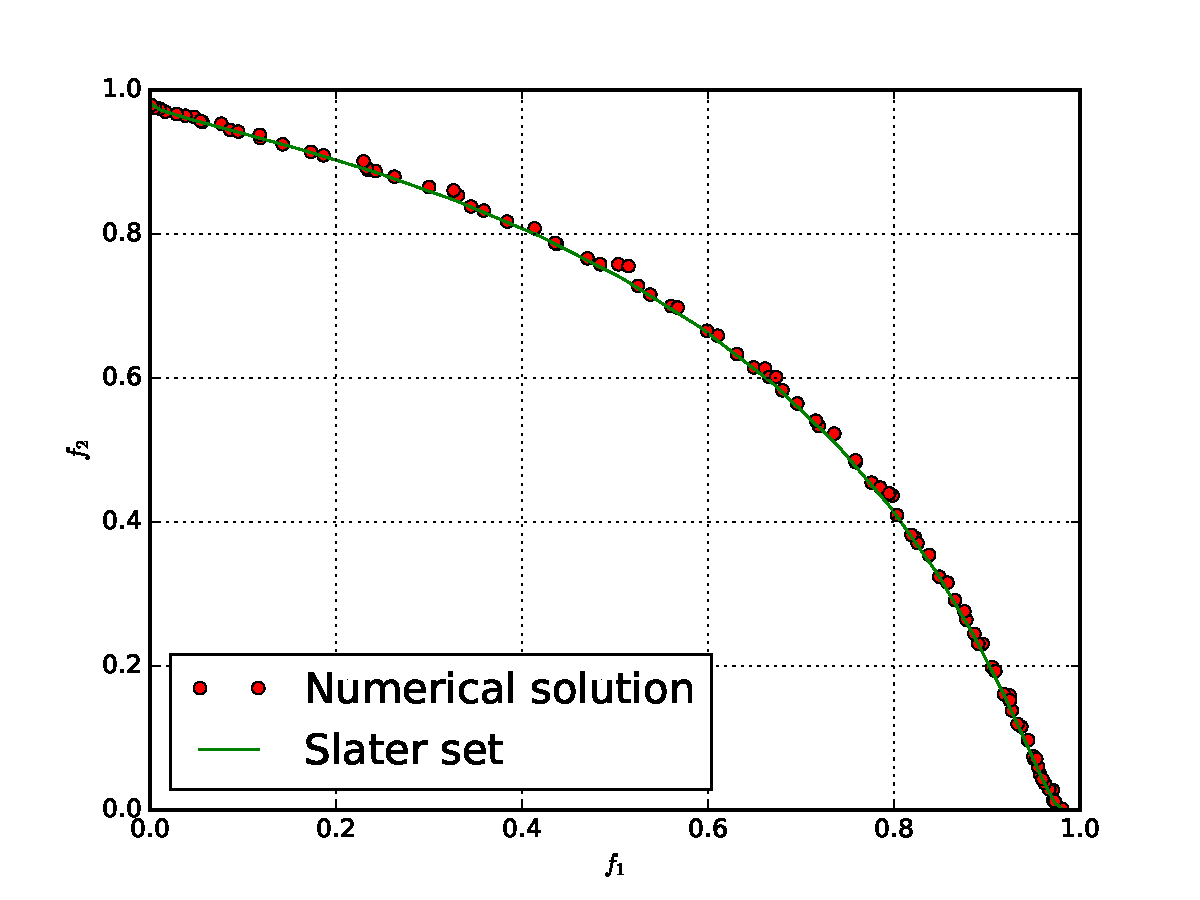
\includegraphics[width=.5\textwidth]{img/fonseca_glob.pdf} }}
    \subfloat[MOLF with \(q=4\)]{{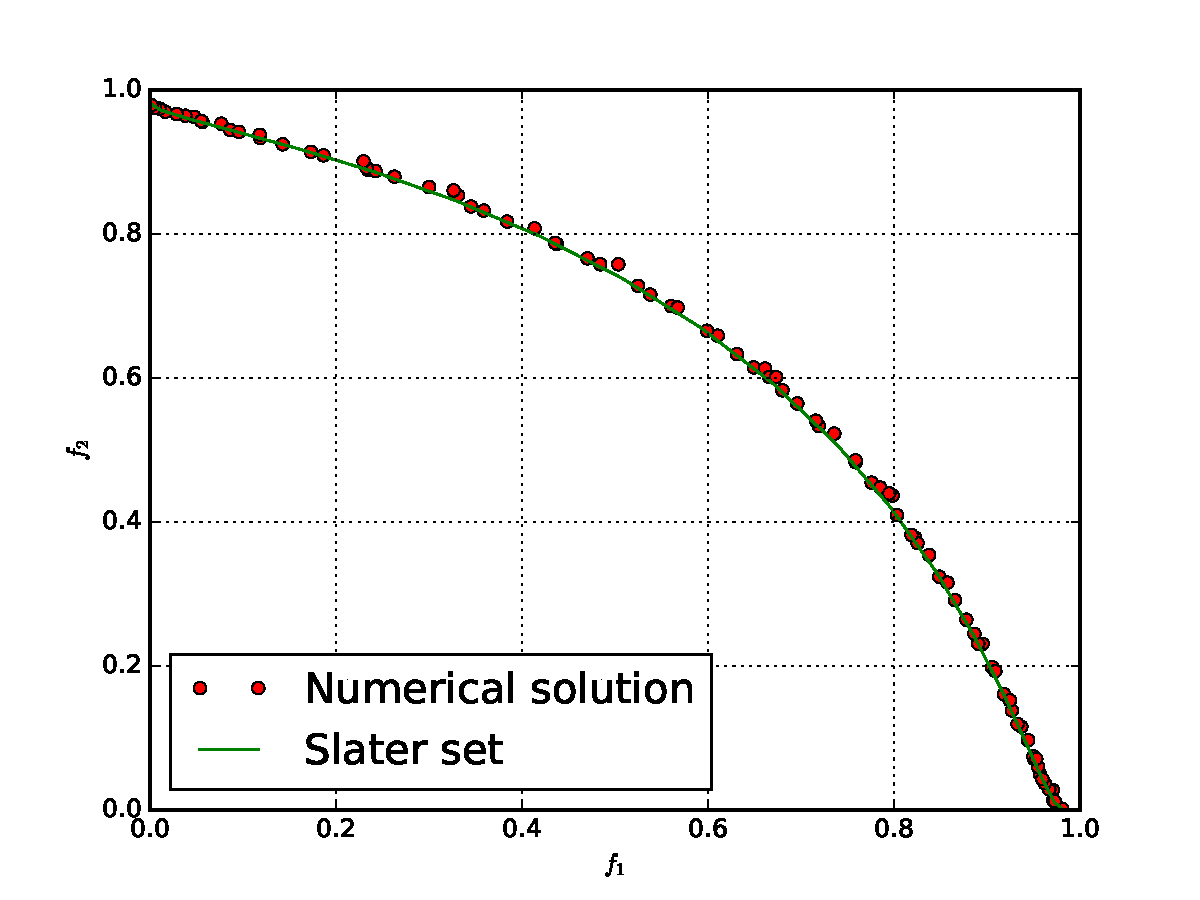
\includegraphics[width=.5\textwidth]{img/fonseca_loc.pdf} }}
    \caption{Numericas estimation of \(S\) obtained by MOLF}
    \label{fig:fonseca_slater}
\end{figure}

В дальнейшем для всех экспериментов будем использовать MOLF при \(q=4\).
\paragraph{Parallel method results.} Чтобы продемонстрировать ускорение по итерациям, которое даёт MOLF при \(p > 1\), были решены все задачи из секции \ref{sec:test_problems} при значениях \(p=1,2,4,8,16\). Параметры метода при этом были следующие: \(r=4.5\), \(\varepsilon=0.01\), \(\alpha=15\). Для задачи (\ref{eq:schaffer2}) \(\varepsilon=0.001\). В таблице \ref{tab:exResultsIters} приведено количество итераций (в скобках мощность оценки множества \(S\)), а в таблице \ref{tab:exResultsItersSpeedup} --- ускорение по итерациям.

Как видно из таблицы \ref{tab:exResultsIters}, мощность оценки множества \(S\) при изменении \(p\) меняется незначительно, т. е. качество полученной оценки сохраняется. В то же время, количество итераций соркащается пропорционально увеличению значения \(p\) (таблица \ref{tab:exResultsItersSpeedup}). На рис. \ref{fig:s_estimation_all} приведены примеры численных решений рассматриваемых задач.
\begin{table}
  \centering
  \caption{Results of numerical experiments: number of iterations iterations}
  \label{tab:exResultsIters}
  \begin{tabular}{|l|K{1.7cm}|K{1.7cm}|K{1.7cm}|K{1.7cm}|K{1.7cm}|}
\hline
\textbf{Problem} & \multicolumn{5}{c|}{\(p\)}\\
\cline{2-6}
  & \(1\) & \(2\) & \(4\) & \(8\) & \(16\)\\
\hline
Markin-Strongin & 1041(198) & 516(198) & 256(185) & 131(197) & 68(191) \\
\hline
Fonseca and Fleming 2d & 1181(93) & 636(99) & 386(111) & 176(95) & 106(97) \\
\hline
Fonseca and Fleming 3d & 5346(160) & 3551(183) & 1186(143) & 606(153) & 351(142) \\
\hline
Schaffer function N. 2 & 271(158) & 136(163) & 64(146) & 32(142) & 16(141)\\
\hline
Poloni's function & 3351(102) & 1706(90) & 856(88) & 426(96) & 201(99) \\
\hline
\end{tabular}
\end{table}

\begin{table}
  \centering
  \caption{Results of numerical experiments: speedup in iterations}
  \label{tab:exResultsItersSpeedup}
  \begin{tabular}{|l|K{1.5cm}|K{1.5cm}|K{1.5cm}|K{1.5cm}|}
\hline
\textbf{Problem} & \multicolumn{4}{c|}{\(p\)}\\
\cline{2-5}
  & \(2\) & \(4\) & \(8\) & \(16\)\\
\hline
Markin-Strongin & 2.02 & 4.07 & 7.95 & 15.31 \\
\hline
Fonseca and Fleming 2d & 1.86 & 3.06 & 6.71 & 11.14 \\
\hline
Fonseca and Fleming 3d & 1.51 & 4.51 & 8.82 & 15.23 \\
\hline
Schaffer problem N. 2 & 1.99 & 4.23 & 8.47 & 16.94\\
\hline
Poloni's problem & 1.96 & 3.91 & 7.87 & 16.67 \\
\hline
\end{tabular}
\end{table}

\begin{figure}[ht]
    \centering
    \subfloat[Markin-Strongin problem]{{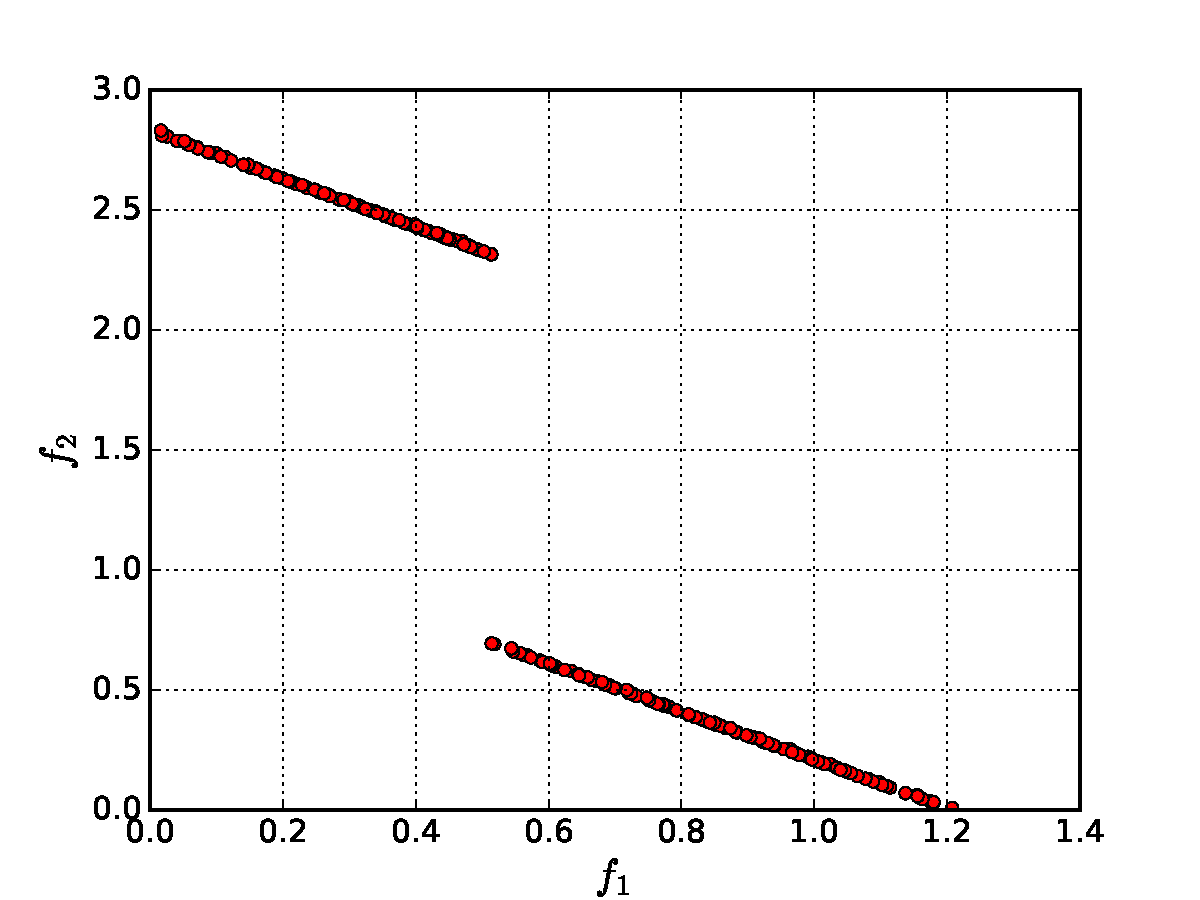
\includegraphics[width=.5\textwidth]{img/strongin.pdf} }}
    \subfloat[Fonseca and Fleming 3d problem]{{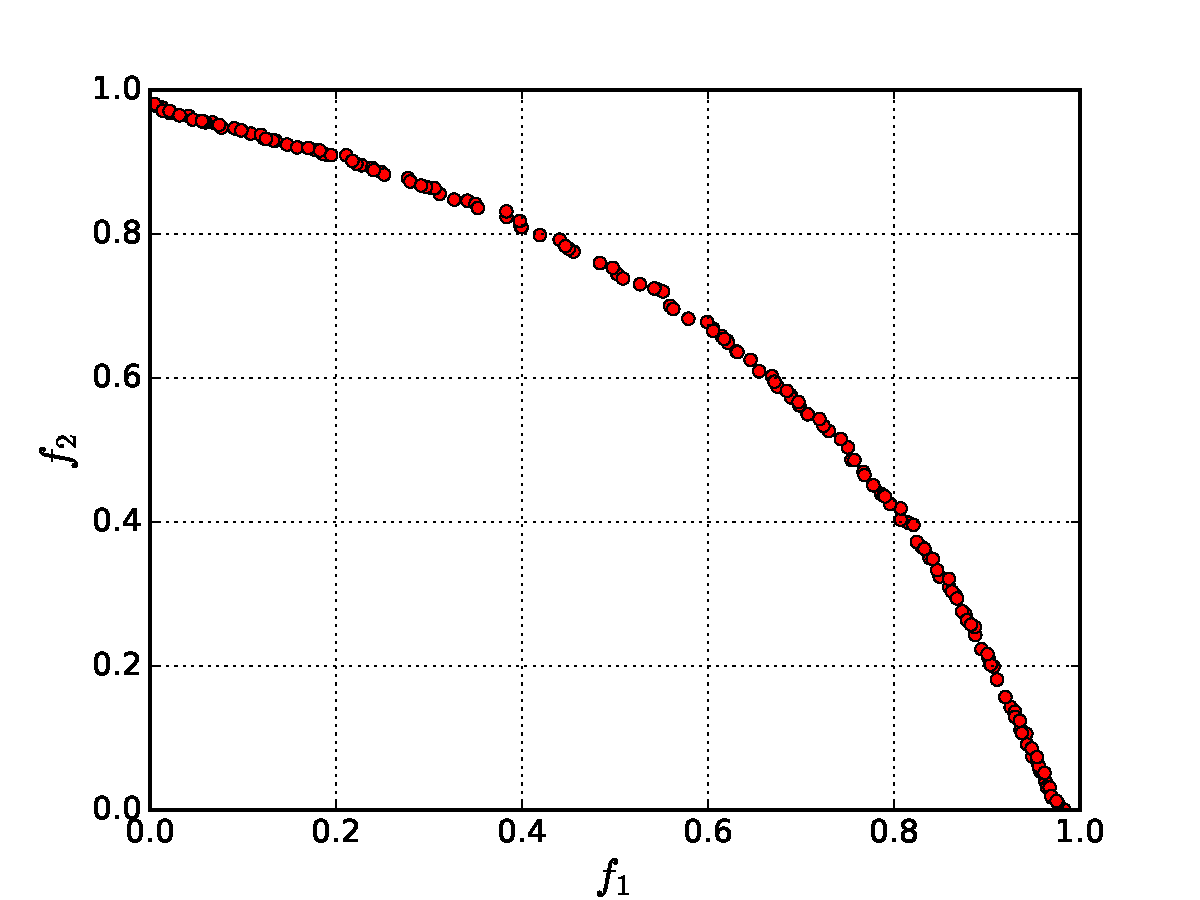
\includegraphics[width=.5\textwidth]{img/fonseca.pdf} }}

    \subfloat[Schaffer problem N. 2]{{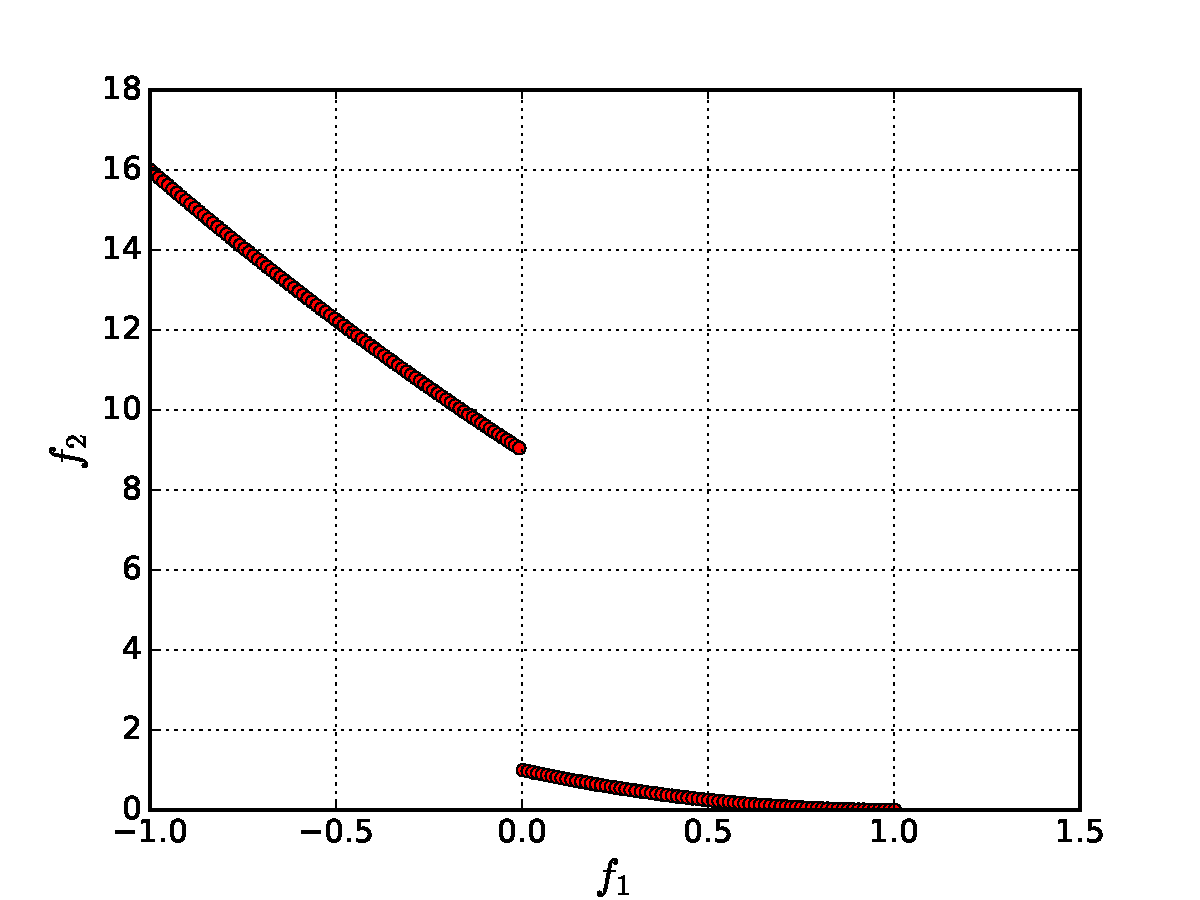
\includegraphics[width=.5\textwidth]{img/schaffer2.pdf} }}
    \subfloat[Poloni's problem]{{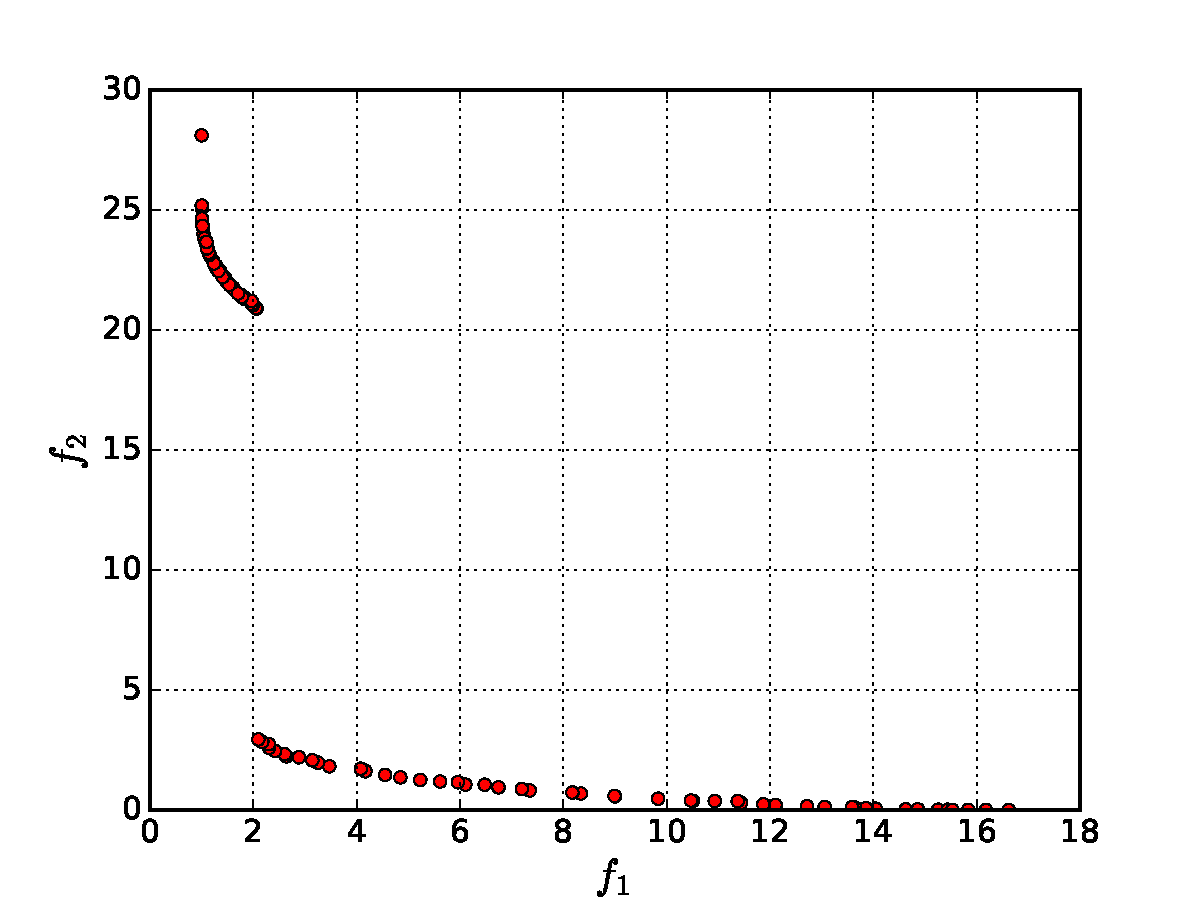
\includegraphics[width=.5\textwidth]{img/poloni.pdf} }}
    \caption{Numericas estimation of \(S\) obtained by MOLF}
    \label{fig:s_estimation_all}
\end{figure}

\paragraph{Parallel method time speedup.} Целевые функции всех перечисленных в разделе задачи обладают невысокой вычислительной сложностью. Чтобы продемонстрировать возможность получения ускорения по времени для задач с трудновычислимыми критериями, в критерии были внесены дополнительные интенсивные вычисления с плавающей точкой, не влияющие на результирующие значения. Полученные при этом ускорения приведены в таблице \ref{tab:exResultsTimeSpeedup}. Ускорение по времени во всех случаях меньше, чем ускорение по итерациям, т.к. часть времени выполнения занимает работа метоад оптимизации, однако распареллеливание в большинстве случаев довольно эффективно и в случае 16 рабочих потоков. При ещё большей вычислительной сложности критериев стоит ожидать увеличения ускорения по времени для большого числа потоков.

\begin{table}[ht]
  \centering
  \caption{Results of numerical experiments: speedup in time}
  \label{tab:exResultsTimeSpeedup}
  \begin{tabular}{|l|K{1.5cm}|K{1.5cm}|K{1.5cm}|K{1.5cm}|K{1.5cm}|}
\hline
\textbf{Problem} & \multicolumn{5}{c|}{\(p\)}\\
\cline{2-6}
&\(1\)(time, s) & \(2\) & \(4\) & \(8\) & \(16\)\\
\hline
Markin-Strongin & 104.47 & 1.97 & 3.65 & 6.79 & 9.90 \\
\hline
Fonseca and Fleming 2d & 118.95 & 1.85 & 2.81 & 5.79 & 6.40 \\
\hline
Fonseca and Fleming 3d & 554.45 & 1.51 & 4.14 & 8.05 & 10.69 \\
\hline
Schaffer problem N. 2 & 27.21 & 1.91 & 3.79 & 6.39 & 6.37\\
\hline
Poloni's problem & 336.74 & 1.82 & 3.64 & 6.98 & 10.60 \\
\hline
\end{tabular}
\end{table}

\section{Conclusion}
В работе был рассмотрен метод решения многокритериальных задач оптимизации, позволяющий находить равномерную оценку множества слабо-оптимальных точек. К нему применены техники распараллеливания и ускорения сходимости, общие для всех алгоритмов подобного структуры \cite{strOptBook}, chapter 3. Проведённые численные эксперименты показали наличие ускорения сходимости при использовании local refinement. Также для данного метода оказалось эффективным распареллеливание по характеристикам. Как и для информационных методов скалярной оптимизации, ускорение по итерациям при распареллеливании по характеристикам оказывается линейным в большинстве случаев \cite{barkalovLebedef2016}. Исходя из результатов эскпериментов, параллельный MOLF применим в задачах низкой размерности с трудновычислимыми критериями.
%
% ---- Bibliography ----
%
%\bibliographystyle{plain}
%\bibliographystyle{alpha}
\bibliographystyle{unsrt}
%\bibliographystyle{splncs03}
\bibliography{u_pdc_refs}

\clearpage
\addtocmark[2]{Author Index} % additional numbered TOC entry
\renewcommand{\indexname}{Author Index}
\printindex
\clearpage
\end{document}
